% !TeX program = lualatex
% !TeX spellcheck = uk_UA

\documentclass[14pt, a4paper]{extarticle}

% --- Мови та шрифти (згідно з ДСТУ) ---
\usepackage{fontspec}
\usepackage[english, ukrainian]{babel}
\usepackage{csquotes}

\setmainfont{Times New Roman}
\setsansfont{Arial}
\setmonofont{Courier New}[Scale=0.85]

% --- Математичні пакети ---
\usepackage{amsmath, amssymb, mathtools}

% --- Оптимізація тексту для LuaLaTeX ---
\usepackage[protrusion=true, expansion=true]{microtype}
\emergencystretch=1.5em

% --- Параметри сторінки згідно з ДСТУ 3008:2015 ---
\usepackage[
    left=30mm,
    right=15mm,
    top=20mm,
    bottom=20mm,
    footskip=10mm,
    headheight=17pt
]{geometry}

% --- Міжрядковий інтервал (еквівалент 1.5 Word) та абзацний відступ ---
\linespread{1.3}
\usepackage{indentfirst}
\setlength{\parindent}{1.25cm}
\setlength{\parskip}{0pt}

% --- Колонтитули та нумерація сторінок (вгорі праворуч, без лінійок) ---
\usepackage{fancyhdr}
\fancypagestyle{plain}{
    \fancyhf{}
    \rhead{\thepage}
    \renewcommand{\headrulewidth}{0pt}
}
\pagestyle{plain}

% --- Форматування заголовків згідно з ДСТУ 3008:2015 ---
\usepackage[explicit]{titlesec}

% Формат розділів (14pt, напівжирний, абзацний відступ 1.25cm, без відступу праворуч)
\titleformat{\section}[block]
{\normalsize\bfseries\raggedright}
{\thesection\ }
{0pt}
{#1}
\titlespacing*{\section}{\parindent}{14pt}{7pt}

% Формат підрозділів
\titleformat{\subsection}[block]
{\normalsize\bfseries\raggedright}
{\thesubsection\ }
{0pt}
{#1}
\titlespacing*{\subsection}{\parindent}{14pt}{7pt}

% --- Списки (компактні, вирівняні за абзацним відступом) ---
\usepackage{enumitem}
\setlist{
    nosep,
    leftmargin=*,
    labelindent=\parindent
}
\setlist[itemize]{label=---}

% --- Підписи до рисунків та таблиць згідно з ДСТУ 3008:2015 ---
\usepackage{caption}
\usepackage{subcaption}
\DeclareCaptionLabelSeparator{emdash}{ — }

\captionsetup[figure]{
    labelsep=emdash,
    name={Рисунок},
    justification=centering,
    position=bottom,
    font=normalsize
}

\captionsetup[table]{
    labelsep=emdash,
    name={Таблиця},
    justification=raggedright,
    singlelinecheck=false,
    position=top,
    font=normalsize
}

\captionsetup[sub]{
    font=small,
    labelformat=simple,
    labelsep=space
}
\renewcommand\thesubfigure{(\alph{subfigure})}

% --- Таблиці (книжковий стиль, нормальний інтервал) ---
\usepackage{booktabs}
\renewcommand{\arraystretch}{1.0}

% --- Фрагменти коду ---
\usepackage{xcolor}
\usepackage{listings}
\lstset{
    basicstyle=\ttfamily\scriptsize\linespread{1.0}\selectfont,
    breaklines=true,
    breakatwhitespace=true,
    columns=fullflexible,
    frame=single,
    numbers=left,
    numberstyle=\tiny\color{gray},
    keywordstyle=\color{blue!80!black}\bfseries,
    commentstyle=\color{green!50!black}\itshape,
    stringstyle=\color{red!70!black},
    showstringspaces=false,
    tabsize=4,
    xleftmargin=1.25cm
}

% --- Графіка та гіперпосилання ---
\usepackage{graphicx}
\usepackage[hidelinks]{hyperref}

% --- Додатки згідно з ДСТУ 3008:2015 (українські літери) ---
\makeatletter
\newcommand{\ukralph}[1]{\expandafter\@ukralph\csname c@#1\endcsname}
\newcommand{\@ukralph}[1]{%
    \ifcase#1\or А\or Б\or В\or Г\or Д\or Е\or Ж\or И\or К\or Л\or М\or Н\or П\or Р\or С\or Т\or У\or Ф\or Х\or Ц\or Ш\or Щ\or Ю\or Я\else\@ctrerr\fi}
\makeatother

\newcommand{\setupappendices}{
    \setcounter{section}{0}
    \renewcommand{\thesection}{ДОДАТОК \ukralph{section}}
    \titleformat{\section}[block]
    {\normalsize\bfseries\centering}
    {}
    {0pt}
    {\MakeUppercase{##1}}
    \titlespacing*{\section}{0pt}{14pt}{7pt}
}

% --- Завантаження модуля обробки таблиць Lua ---
\directlua{dofile("tables.lua")}

\begin{document}

% --- Титульна сторінка ---
\begin{titlepage}
    \thispagestyle{empty}
    \setlength{\parindent}{0pt}
    
    % --- ШАПКА ДОКУМЕНТА (12pt, напівжирний) ---
    \begin{center}
        {\fontsize{12pt}{16pt}\selectfont\bfseries
        МІНІСТЕРСТВО ОСВІТИ І НАУКИ УКРАЇНИ\\[3pt]
        ОДЕСЬКИЙ НАЦІОНАЛЬНИЙ УНІВЕРСИТЕТ ІМЕНІ І.І. МЕЧНИКОВА\\[3pt]
        ФАКУЛЬТЕТ МАТЕМАТИКИ, ФІЗИКИ ТА ІНФОРМАЦІЙНИХ ТЕХНОЛОГІЙ\\[3pt]
        КАФЕДРА ОПТИМАЛЬНОГО КЕРУВАННЯ ТА ЕКОНОМІЧНОЇ КІБЕРНЕТИКИ\par}
    \end{center}

    \vspace{1.5cm}

    % --- НАЗВА РОБОТИ ТА ТЕМА ---
    \begin{center}
        {\fontsize{18pt}{22pt}\selectfont\bfseries ЗВІТ\\
        до лабораторної роботи № 1\par}
        \vspace{0.4cm}
        {\fontsize{14pt}{18pt}\selectfont
        з дисципліни «Системи комп’ютерного зору»\par}
        \vspace{0.4cm}
        {\fontsize{16pt}{20pt}\selectfont\bfseries
        на тему:\\[6pt]
        «Середовище, подання зображень, колірні простори»\par}
    \end{center}

    \vspace{1.5cm}

    % --- ПРАВИЙ БЛОК (Виконавець, керівник) ---
    \hfill
    \begin{minipage}{0.60\textwidth}
        \raggedright
        {\fontsize{14pt}{19pt}\selectfont
        Виконав:\\[2pt]
        студент 3 курсу групи 1\\[2pt]
        спеціальності F1 «Прикладна математика»\\[2pt]
        Касьянов Ярослав Володимирович
        
        \vspace{0.8cm}
        
 
        }
    \end{minipage}

    \vfill

    % --- МІСТО ТА РІК ---
    \begin{center}
        {\fontsize{12pt}{14pt}\selectfont\bfseries Одеса --- 2026\par}
    \end{center}
\end{titlepage}

% За ДСТУ титульна сторінка входить у загальну нумерацію як 1-ша, 
% тому наступна сторінка отримує номер 2:
\setcounter{page}{2}


\section{Мета роботи}
Ознайомлення з базовими структурами представлення растрових зображень у бібліотеці OpenCV та середовищі Python; дослідження особливостей 8-бітного кодування (\texttt{uint8}) і наслідків арифметичного переповнення; експериментальна оцінка втрат інформації при стисненні; аналіз службових метаданих EXIF; дослідження поведінки й стійкості порогової сегментації в колірних просторах RGB та HSV за зміни спектрального складу освітлення; дослідження просторового аліасингу (теорема Найквіста), методів інтерполяції та нелінійних радіометричних ефектів гамма-кодування; формування та верифікація власного набору з 20 зображень.

\section{Вихідні дані}
\begin{itemize}
    \item \textbf{Апаратне забезпечення}: смартфон Google Pixel 5. Основна камера: фізична фокусна відстань $f = 4.38$~мм ($27$~мм в еквіваленті 35-мм), діафрагма $f/1.73$, оптичний сенсор $1/2.55''$ (розмір пікселя $1.4$~мкм).
    \item \textbf{Вхідні зображення (\texttt{lab01/data/})}:
    \begin{itemize}
        \item \textbf{Частина A}: \texttt{A/photo.jpg} --- високодеталізований знімок сакури на фоні неба ($2268 \times 4032$, 3 канали, \texttt{uint8}, витримка $1/4673$~с, ISO~69).
        \item \textbf{Частина B}: \texttt{B/day\_light.png} (денне світло біля вікна, $T_c \approx 6000$~K, витримка $1/234$~с, ISO~61) та \texttt{B/lamp\_light.png} (лампа розжарювання ввечері, $T_c \approx 2700$~K, витримка $1/25$~с, ISO~557). Об'єкт --- жорсткий диск (HDD 3.5''). Для обох кадрів створено ручні бінарні еталонні маски (\texttt{day\_light\_mask.png}, \texttt{lamp\_light\_mask.png}); площа об'єкта становить $34.20\%$ на кадрі 1 та $39.84\%$ на кадрі 2.
        \item \textbf{Частина C}: \texttt{C/texture.png} --- дрібнозерниста текстура столу ($2268 \times 4032$, 3 канали).
        \item \textbf{Домашнє завдання}: \texttt{Homework/} --- 20 знімків реальної сцени: 10 ракурсів повороту камери (\texttt{angle1}--\texttt{angle10}), 5 знімків різного масштабу (\texttt{scale1}--\texttt{scale5}) та 5 знімків різного освітлення (\texttt{light1}--\texttt{light5}).
    \end{itemize}
\end{itemize}

\section{Теоретичні відомості}
\begin{enumerate}
    \item \textbf{MSE та PSNR} для триканальних зображень розміром $H \times W$:
    \begin{align}
        \text{MSE} &= \frac{1}{3 H W} \sum_{c=1}^3 \sum_{y=0}^{H-1} \sum_{x=0}^{W-1} \left(I_1(y, x, c) - I_2(y, x, c)\right)^2, \\
        \text{PSNR} &= 10 \cdot \log_{10} \left( \frac{255^2}{\text{MSE}} \right) \quad [\text{дБ}].
    \end{align}
    Для тотожних масивів ($\text{MSE} = 0$) величина $\text{PSNR} = +\infty$.

    \item \textbf{Метрики бінарної сегментації} (порівняння прогнозу $P$ з еталоном $GT$):
    \begin{equation}
        \text{Accuracy} = \frac{TP + TN}{TP + TN + FP + FN},
        \\
         \text{IoU} = \frac{|P \cap GT|}{|P \cup GT|} = \frac{TP}{TP + FP + FN}.
    \end{equation}
    Метрика $\text{Accuracy}$ спотворюється дисбалансом класів (прогноз «усе тло» дає точність $65.8\%$), тому об'єктивним критерієм якості є $\text{IoU}$.

    \item \textbf{Колірний простір HSV в OpenCV}: канал відтінку $H \in [0, 179]$ ($H_{\text{deg}} / 2$), насиченість $S \in [0, 255]$, яскравість $V = \max(R,G,B) \in [0, 255]$. При $S \to 0$ координата $H$ втрачає математичну стійкість через сингулярність в ахроматичній точці.

    \item \textbf{Теорема Найквіста та аліасинг}: при децимації зображення у $F$ разів гранична частота становить $f_N = 0.5$~цикл/пк нової сітки. Просторові гармоніки з $f > f_N$ утворюють хибні низькочастотні гармоніки муару $f_{\text{alias}} = |f - 1.0|$. Для усунення аліасингу застосовують фільтрацію низьких частот (гаусове розмиття із $\sigma \approx 0.5 \cdot F$).

    \item \textbf{Нелінійність гамма-кодування}: у стандарті sRGB яскравість кодується як $V \propto L^{1/\gamma}$ ($\gamma \approx 2.2$). Лінійне усереднення двох пікселів з кодами $a$ та $b$ не дорівнює алгебраїчному середньому їхніх кодів:
    \begin{equation}
        \bar{V}_{\text{naive}} = \frac{a + b}{2} \ne \bar{V}_{\text{correct}} = 255 \cdot \left( \frac{(a/255)^\gamma + (b/255)^\gamma}{2} \right)^{1/\gamma}.
    \end{equation}
\end{enumerate}

\section{Хід роботи}
\begin{enumerate}
    \item \textbf{Частина A (Подання зображення)}: завантажено \texttt{A/photo.jpg} функцією \texttt{cv2.imread}; порівняно виведення BGR проти RGB у \texttt{matplotlib}; промодельовано переповнення \texttt{uint8} при операції \texttt{img + 50} та коректне насичення через \texttt{cv2.add}; збережено знімки у PNG та JPEG ($Q \in \{95, 75, 50, 25, 10\}$), обчислено bpp і PSNR; вилучено метадані EXIF бібліотекою \texttt{Pillow}.
    \item \textbf{Частина B (Колірні простори)}: знято жорсткий диск за денного та лампового освітлення; створено еталонні бінарні маски; реалізовано покоординатний пошук оптимальних меж по 3 каналах у просторах RGB та HSV за критерієм максимуму $\text{IoU}$ на кадрі 1; застосовано знайдені пороги без змін до кадру 2 та виміряно втрату якості.
    \item \textbf{Частина C (Геометрія та радіометрія)}: текстуру \texttt{C/texture.png} зменшено в 4 рази методом \texttt{INTER\_NEAREST} та \texttt{GaussianBlur} ($\sigma = 2.0$) + \texttt{INTER\_NEAREST}; розраховано спектри Фур'є для гармонійної решітки ($T = 6$~пк); масштабовано у 8 разів 3 фрагменти \texttt{photo.jpg} чотирма методами інтерполяції; досліджено вплив гамма-корекції ($\gamma \in \{0.5, 1.0, 2.2\}$) та похибку наївного усереднення при зменшенні.
    \item \textbf{Домашнє завдання}: сформовано та верифіковано набір із 20 кадрів; для кожного виміряно витримку, ISO, дисперсію лапласіана (різкість) та кількість кутових точок FAST; для поворотних пар оцінено взаємне перекриття за гомографією RANSAC над дескрипторами ORB.
\end{enumerate}

\section{Результати експериментів}

\subsection{Частина A: Порядок каналів, переповнення цілих типів та компресія}

\begin{figure}[htbp]
    \centering
    \begin{subfigure}[b]{0.48\textwidth}
        \centering
        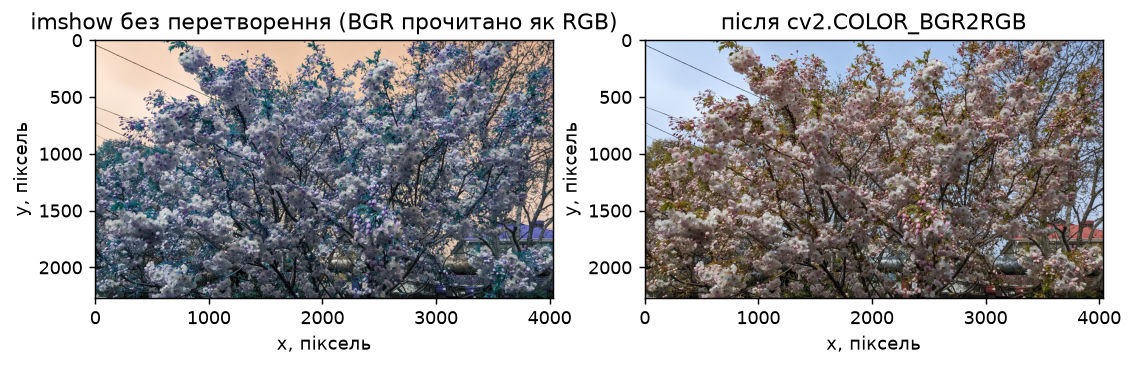
\includegraphics[width=\textwidth]{../figures/a_bgr_vs_rgb.png}
        \caption{Порядок каналів: зліва BGR, справа RGB}
        \label{fig:bgr_rgb}
    \end{subfigure}
    \hfill
    \begin{subfigure}[b]{0.48\textwidth}
        \centering
        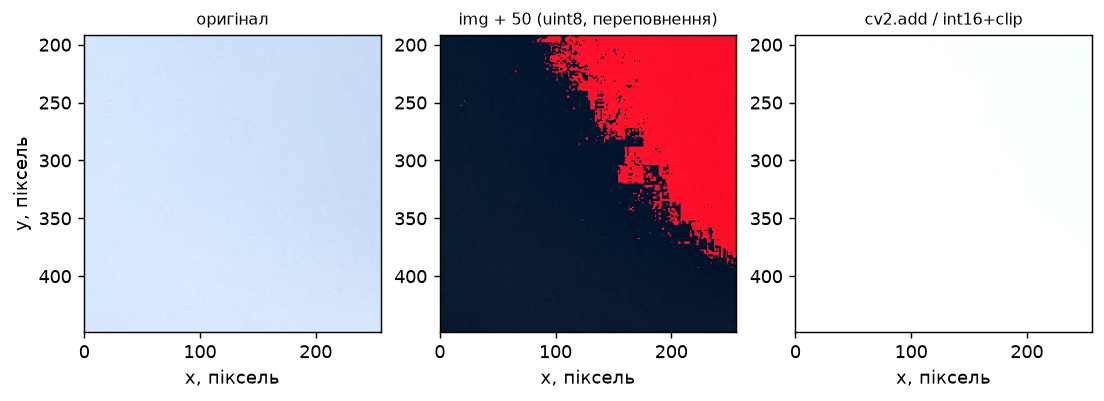
\includegraphics[width=\textwidth]{../figures/a_overflow.png}
        \caption{Переповнення \texttt{uint8} проти насичення}
        \label{fig:overflow}
    \end{subfigure}
    \caption{Особливості представлення та кодування зображень у бібліотеці OpenCV}
\end{figure}

На рисунку~\ref{fig:bgr_rgb} виведення BGR без конвертації спричиняє інверсію колірних координат: синє небо стає пісочно-червоним, а рожеві пелюстки --- синіми. На рисунку~\ref{fig:overflow} операція \texttt{img + 50} над типом \texttt{uint8} призводить до переповнення за модулем 256: $728\,173$ пікселі ($7.96\%$) переповнилися, а $1\,103\,104$ пікселі ($12.06\%$) із вихідною яскравістю $\ge 200$ перетворилися на темні точки ($< 100$), породивши плямистий артефакт на небі.

\begin{table}[htbp]
\centering
\caption{Порівняльний аналіз стиснення знімків \texttt{photo.jpg} та \texttt{day\_light.png}}
\label{tab:compress}
\footnotesize\linespread{1.0}\selectfont
\setlength{\tabcolsep}{3.5pt}
\begin{tabular}{lcccccc}
\toprule
\textbf{Формат / Q} & \multicolumn{3}{c}{\textbf{A/photo.jpg (деталізований сюжет)}} & \multicolumn{3}{c}{\textbf{B/day\_light.png (об'єкт на площині)}} \\
\cmidrule(lr){2-4} \cmidrule(lr){5-7}
& Розмір, КіБ & bpp & PSNR, дБ & Розмір, КіБ & bpp & PSNR, дБ \\
\midrule
\directlua{tab_compression()}
\bottomrule
\end{tabular}
\end{table}

\begin{figure}[htbp]
    \centering
    \begin{subfigure}[b]{0.46\textwidth}
        \centering
        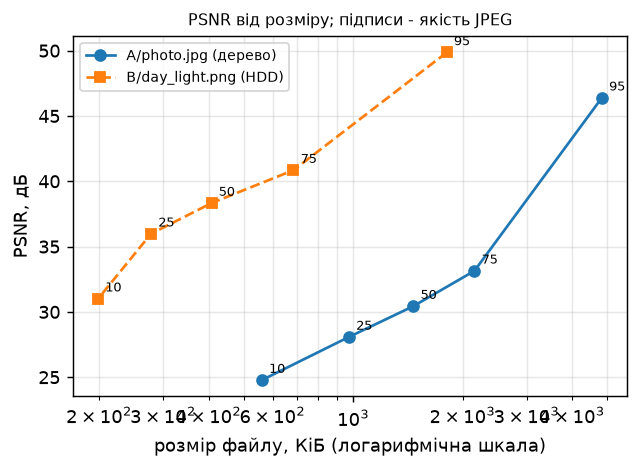
\includegraphics[width=\textwidth]{../figures/a_psnr_vs_size.png}
        \caption{Залежність PSNR від розміру файлу}
    \end{subfigure}
    \hfill
    \begin{subfigure}[b]{0.52\textwidth}
        \centering
        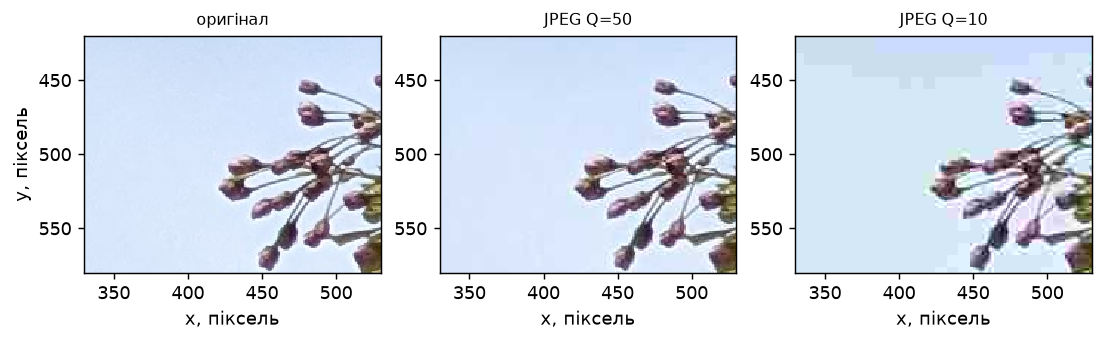
\includegraphics[width=\textwidth]{../figures/a_jpeg_artifacts.png}
        \caption{Артефакти JPEG при $Q=50$ та $Q=10$}
    \end{subfigure}
    \caption{Дослідження ефективності стиснення та компресійних артефактів JPEG}
    \label{fig:compression}
\end{figure}

З таблиці~\ref{tab:compress} та рисунка~\ref{fig:compression} видно, що компресія JPEG при $Q=95$ забезпечує збереження високої якості ($\text{PSNR} = 46.39$~дБ) при скороченні розміру у $3.9$ раза (до $4.33$~bpp) відносно вихідного PNG ($16.97$~bpp). При зниженні якості до $Q=10$ бітрейт падає до $0.50$~bpp, але дискретне квантування DCT породжує характерну блокову сітку $8 \times 8$ пікселів і граничний дзвін довкола контрастних гілок ($\text{PSNR} = 24.78$~дБ).

\subsection{Частина B: Порогова сегментація та стійкість колірних просторів}

\begin{table}[htbp]
\centering
\caption{Оптимальні порогові інтервали та метрики сегментації при зміні освітлення}
\label{tab:spaces}
\footnotesize\linespread{1.0}\selectfont
\setlength{\tabcolsep}{4pt}
\begin{subtable}[t]{0.43\textwidth}
\centering
\begin{tabular}{lccc}
\toprule
\textbf{Простір} & \textbf{Канал} & \textbf{Кадр 1} & \textbf{Кадр 2} \\
\midrule
\directlua{tab_bounds()}
\bottomrule
\end{tabular}
\caption{Підібрані межі діапазонів}
\end{subtable}
\hfill
\begin{subtable}[t]{0.55\textwidth}
\centering
\begin{tabular}{lccccc}
\toprule
\textbf{Простір} & \multicolumn{2}{c}{\textbf{Кадр 1 (День)}} & \multicolumn{2}{c}{\textbf{Кадр 2 (Лампа)}} & \textbf{Кадр 2*} \\
& Acc & IoU & Acc & IoU & IoU$_{\text{max}}$ \\
\midrule
\directlua{tab_spaces()}
\bottomrule
\end{tabular}
\caption{Метрики перенесення (*підлаштовано)}
\end{subtable}
\end{table}

\begin{figure}[htbp]
    \centering
    \begin{subfigure}[b]{0.63\textwidth}
        \centering
        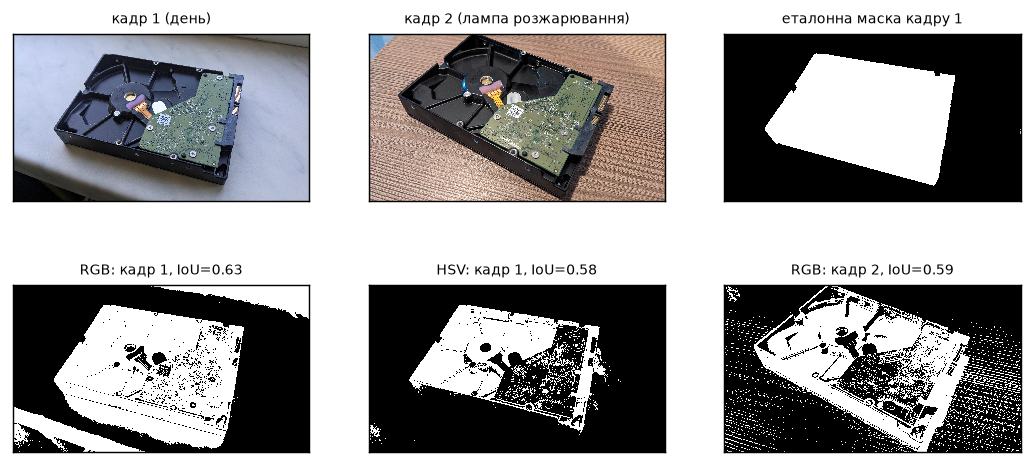
\includegraphics[width=\textwidth]{../figures/b_masks_1.png}
        \caption{Кадри, еталонна маска та результат сегментації в RGB і HSV}
    \end{subfigure}
    \hfill
    \begin{subfigure}[b]{0.35\textwidth}
        \centering
        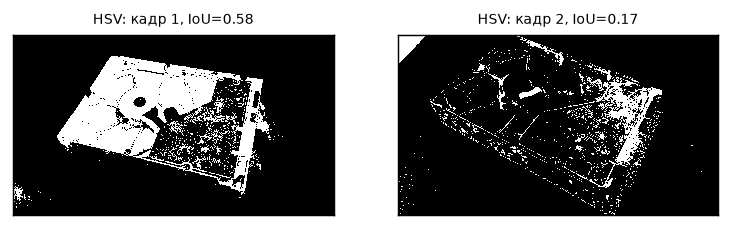
\includegraphics[width=\textwidth]{../figures/b_masks_hsv.png}
        \caption{Маска HSV: день ($\text{IoU}=0.58$) vs лампа ($\text{IoU}=0.17$)}
    \end{subfigure}
    \caption{Порогова бінарна сегментація цільового об'єкта (жорсткого диска)}
    \label{fig:segmentation}
\end{figure}

\begin{figure}[htbp]
    \centering
    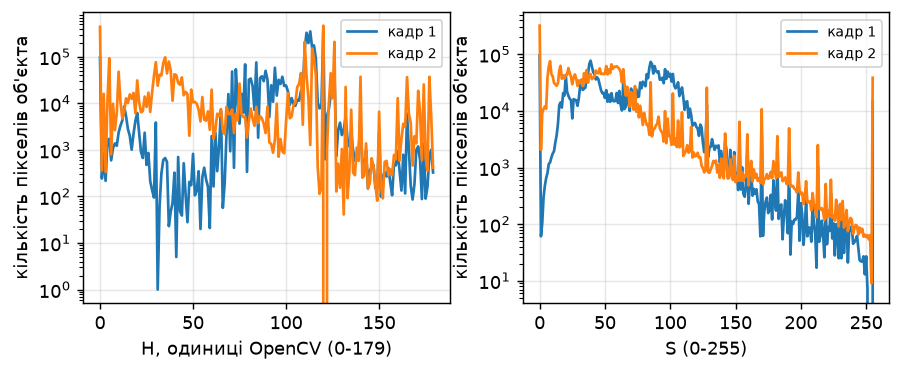
\includegraphics[width=0.76\textwidth]{../figures/b_hsv_hist.png}
    \caption{Гістограми розподілу каналів відтінку $H$ та насиченості $S$ об'єкта в обох кадрах (лог-шкала)}
    \label{fig:hsv_hist}
\end{figure}

Експеримент (таблиця~\ref{tab:spaces}, рисунки~\ref{fig:segmentation}--\ref{fig:hsv_hist}) показав нетривіальну поведінку:
\begin{itemize}
    \item У просторі RGB порогові межі, підібрані на денному світлі, при перенесенні на лампу розжарювання зберігають високу надійність: $\text{IoU}$ знизився лише з $0.6285$ до $0.5885$ (відносне падіння на $6.4\%$).
    \item У просторі HSV перенесення тих самих порогів призвело до падіння $\text{IoU}$ з $0.5783$ до $0.1686$ (падіння на $70.8\%$), а точність склала лише $65.90\%$, що ненабагато перевищує тривіальний класифікатор фону ($60.16\%$).
\end{itemize}

\subsection{Частина C: Геометрія, спектральний аліасинг та радіометрія}

\begin{figure}[htbp]
    \centering
    \begin{subfigure}[b]{0.57\textwidth}
        \centering
        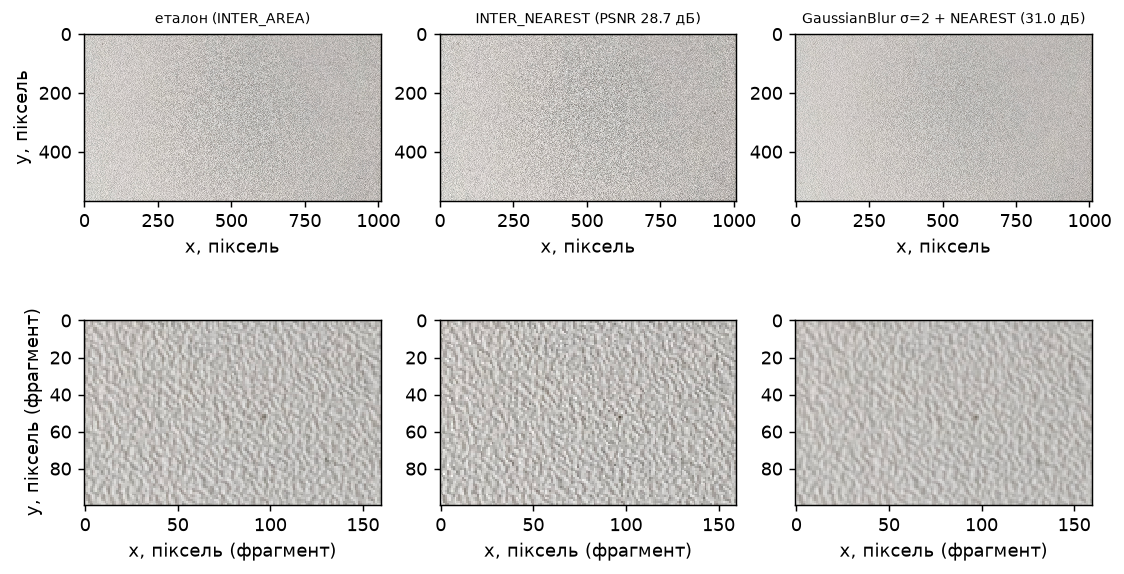
\includegraphics[width=\textwidth]{../figures/c_aliasing_map.png}
        \caption{Зменшення $\times 4$: еталон, NEAREST та Gauss+NEAREST}
    \end{subfigure}
    \hfill
    \begin{subfigure}[b]{0.41\textwidth}
        \centering
        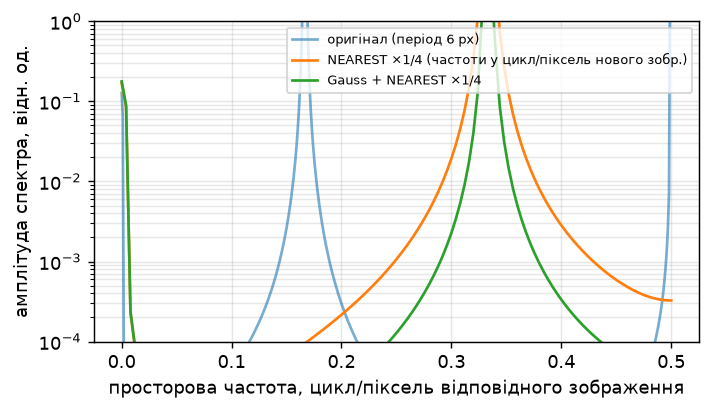
\includegraphics[width=\textwidth]{../figures/c_aliasing_spectrum.png}
        \caption{Спектри решітки $T=6$~пк (лог-шкала)}
    \end{subfigure}
    \caption{Експериментальне підтвердження просторового аліасингу}
    \label{fig:aliasing}
\end{figure}

При зменшенні текстури \texttt{C/texture.png} у 4 рази пряма децимація \texttt{INTER\_NEAREST} забезпечує $\text{PSNR} = 28.71$~дБ відносно \texttt{INTER\_AREA}. Попереднє згладжування фільтром Гаусса ($\sigma = 2.0$) підвищує PSNR до $31.03$~дБ ($+2.32$~дБ). На періодичній структурі ($T = 6$~пк, $f_0 = 0.167$~цикл/пк) частота після проріджування $\times 4$ становить $0.67$~цикл/пк, що перевищує частоту Найквіста ($0.5$). Виникає потужна хибна гармоніка муару на частоті $f = |0.67 - 1.0| = 0.33$~цикл/пк ($T = 3.0$~пк) з амплітудою $39.41$. Гаусовий антиаліасинговий фільтр пригнічує цей паразитний пік у $8.5$ раза (амплітуда $4.64$, рисунок~\ref{fig:aliasing}).

\begin{table}[htbp]
\centering
\caption{Порівняння методів інтерполяції при 8-кратному збільшенні фрагментів (PSNR, дБ)}
\label{tab:interp}
\footnotesize\linespread{1.0}\selectfont
\begin{tabular}{lcccc}
\toprule
\textbf{Метод інтерполяції} & \textbf{Фрагмент 1 (дроти)} & \textbf{Фрагмент 2 (квіти)} & \textbf{Фрагмент 3 (гілки)} & \textbf{Середнє $\pm$ СВ, дБ} \\
\midrule
\directlua{tab_interp()}
\bottomrule
\end{tabular}
\end{table}

\begin{figure}[htbp]
    \centering
    \begin{subfigure}[b]{0.60\textwidth}
        \centering
        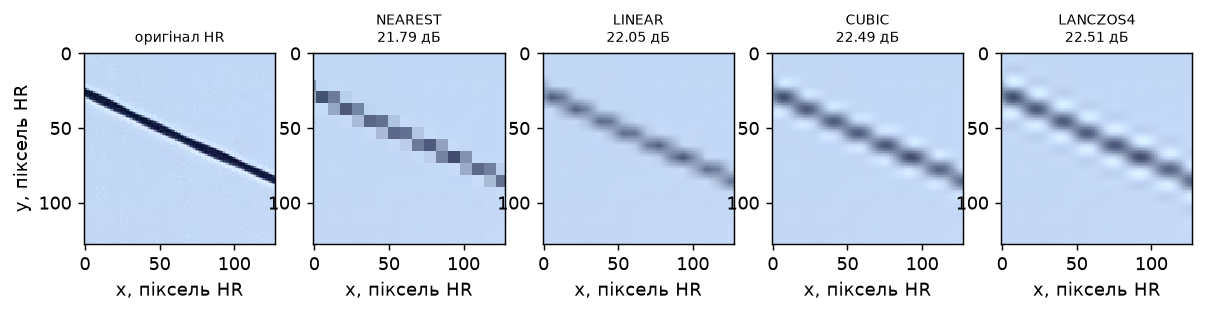
\includegraphics[width=\textwidth]{../figures/c_interpolation.png}
        \caption{Порівняння інтерполяцій тонкого контрастного об'єкта}
    \end{subfigure}
    \hfill
    \begin{subfigure}[b]{0.38\textwidth}
        \centering
        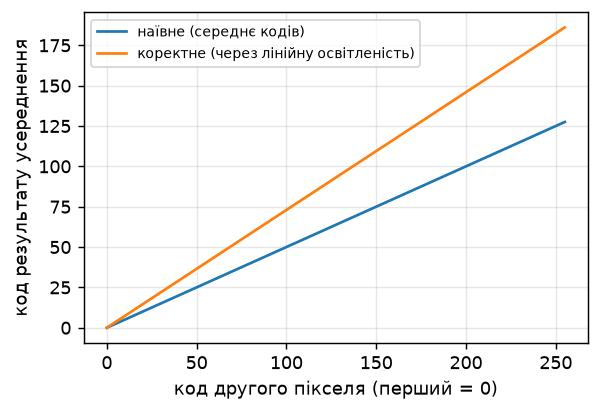
\includegraphics[width=\textwidth]{../figures/c_gamma_average.png}
        \caption{Кодове усереднення проти лінійного}
    \end{subfigure}
    \caption{Дослідження методів інтерполяції та ефектів нелінійності гамма-кодування}
    \label{fig:interp_gamma}
\end{figure}

\begin{figure}[htbp]
    \centering
    \begin{subfigure}[b]{0.60\textwidth}
        \centering
        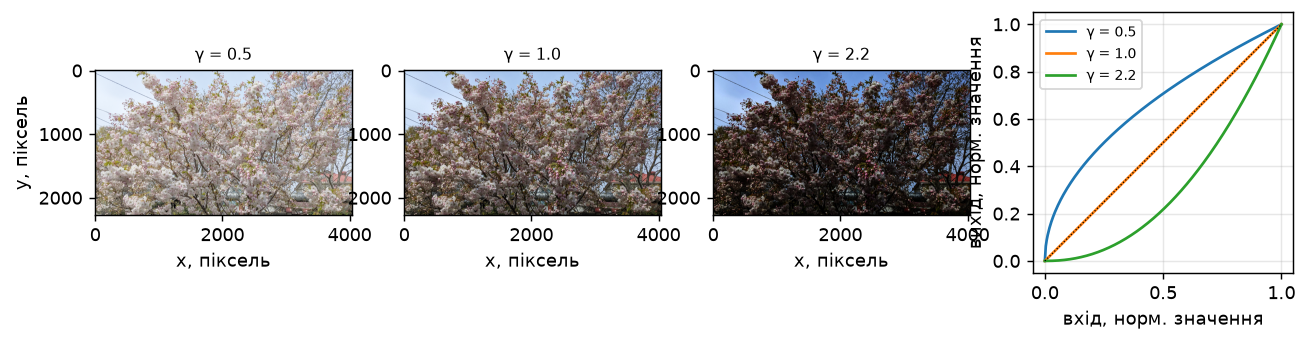
\includegraphics[width=\textwidth]{../figures/c_gamma.png}
        \caption{Трансформація зображення при $\gamma \in \{0.5, 1.0, 2.2\}$}
    \end{subfigure}
    \hfill
    \begin{subfigure}[b]{0.38\textwidth}
        \centering
        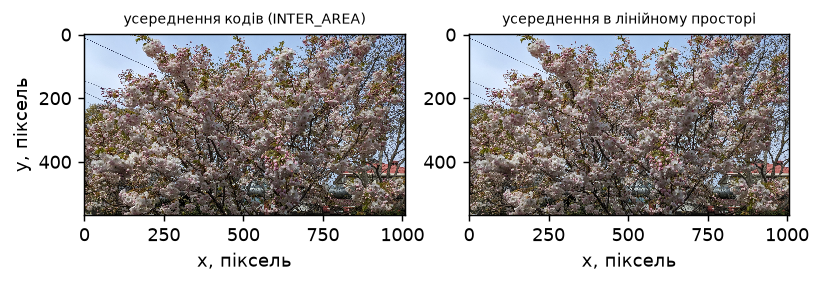
\includegraphics[width=\textwidth]{../figures/c_gamma_downscale.png}
        \caption{Зменшення $\times 4$: коди vs лінійний простір}
    \end{subfigure}
    \caption{Радіометрична дія гамма-корекції на контрастність та яскравість}
    \label{fig:gamma}
\end{figure}

З таблиці~\ref{tab:interp} та рисунка~\ref{fig:interp_gamma} випливає, що кубічна інтерполяція (\texttt{CUBIC}, $20.34$~дБ) та фільтр Ланцоша (\texttt{LANCZOS4}, $20.37$~дБ) суттєво перевершують лінійну ($19.95$~дБ) та східчасту найближчого сусіда ($19.67$~дБ).

На рисунку~\ref{fig:gamma} проілюстровано нелінійність гамма-кодування: наївне середнє кодів $0$ та $255$ дає $127.5$, яскравість якого становить $(127.5/255)^{2.2} = 0.218$ замість $0.500$. Фізично коректний код суміші дорівнює $255 \cdot (0.5)^{1/2.2} = 186.1$. Децимація \texttt{photo.jpg} $\times 4$ безпосередньо у нелінійному sRGB штучно затемнює зображення: середня яскравість знижується з $0.2445$ до $0.2343$, а максимальна похибка сягає $48.7$ градацій на піксель.

\subsection{Домашнє завдання: Верифікація власного набору з 20 зображень}

\begin{figure}[htbp]
    \centering
    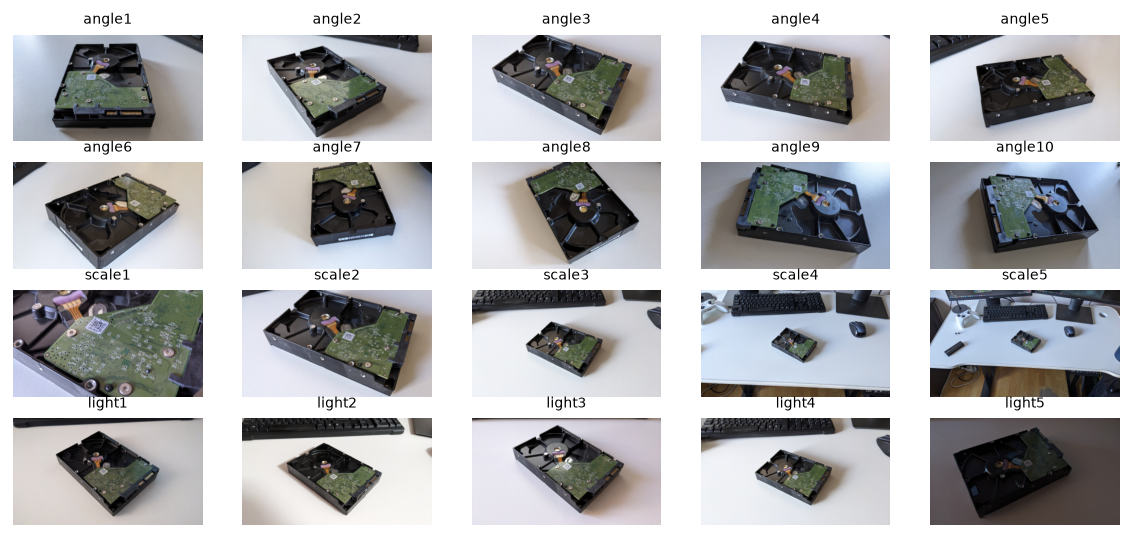
\includegraphics[width=0.90\textwidth]{../figures/hw_contact_sheet.png}
    \caption{Контактний аркуш 20 кадрів власного набору: 10 ракурсів (\texttt{angle}), 5 масштабів (\texttt{scale}), 5 освітлень (\texttt{light})}
    \label{fig:contact_sheet}
\end{figure}

\begin{table}[htbp]
\centering
\caption{Оцінка перекриття сусідніх кадрів поворотної серії (\texttt{angle1}--\texttt{angle10}) через RANSAC-гомографію}
\label{tab:overlap}
\footnotesize\linespread{1.0}\selectfont
\begin{tabular}{lccc}
\toprule
\textbf{Пара сусідніх кадрів} & \textbf{Зіставлень ORB} & \textbf{Інлаєри RANSAC} & \textbf{Розраховане перекриття, \%} \\
\midrule
\directlua{tab_hw_overlap()}
\bottomrule
\end{tabular}
\end{table}

Сусідні кадри поворотної серії (таблиця~\ref{tab:overlap}) мають перекриття від $67.4\%$ до $94.6\%$ (середнє $78.8\%$), що з запасом виконує умову практикуму ($\ge 40\%$). Кожен кадр містить від $1\,660$ до $8\,372$ кутових деталей FAST (вимога «кілька десятків»). Перевірка хеш-сум MD5 виявила, що файли \texttt{scale3.jpg} та \texttt{light4.jpg} є дублікатами (однаковий хеш, експозиція $1/24$~с, ISO~134).

\section{Аналіз результатів}
\begin{enumerate}
    \item \textbf{Причини низької стійкості порогів HSV}:
    Поширена думка про безумовну перевагу простору HSV над RGB при зміні освітлення спростована експериментально: при переході з денного світла на лампу розжарювання $\text{IoU}$ у просторі HSV впав у $3.4$ раза (з $0.5783$ до $0.1686$), тоді як у RGB знизився лише на $6.4\%$ (з $0.6285$ до $0.5885$). Об'єкт містить металеві темні поверхні з низькою насиченістю ($S < 60$). У цій зоні відтінок $H$ є сингулярним і має високу дисперсію під впливом шуму. Зсув спектра лампи розжарювання у теплу ділянку змістив відтінок $H$ металевого шасі нижче порогу $36$, виключивши його з маски. Простір RGB завдяки спільній коваріації каналів виявився стабільнішим.

    \item \textbf{Небезпека операцій над типом \texttt{uint8}}:
    Операція \texttt{img + 50} над цілими числами без знака призводить до переповнення через модульну арифметику $256$. Яскраві ділянки перетворюються на чорні тіні ($255 + 50 \to 49$). У комп'ютерному зорі необхідно використовувати арифметику з насиченням (\texttt{cv2.add}) або проміжне приведення до знакового типу \texttt{int16} з операцією \texttt{np.clip}.

    \item \textbf{Просторовий аліасинг та фільтрація}:
    Просте проріджування решітки без фільтрації низьких частот генерує паразитні низькочастотні гармоніки, чия амплітуда у $8.5$ раза перевищує згладжений сигнал, що є джерелом грубих помилок у детекторах кутів і дескрипторах наступних робіт.
\end{enumerate}

\section{Висновки}
\begin{enumerate}
    \item Стиснення JPEG з $Q=95$ скорочує обсяг даних у $3.9$ раза (з $16.97$ до $4.33$~bpp) за збереження високої якості ($\text{PSNR} = 46.39$~дБ). При $Q=10$ бітрейт падає до $0.50$~bpp, але PSNR деградує до $24.78$~дБ із блоковими артефактами $8 \times 8$ пікселів.
    \item Порогова сегментація у просторі RGB виявилася на порядок стійкішою до зміни колірної температури освітлення (падіння $\text{IoU}$ лише на $6.4\%$, з $0.6285$ до $0.5885$), ніж у просторі HSV, де спостерігалося падіння $\text{IoU}$ на $70.8\%$ (з $0.5783$ до $0.1686$) через нестабільність відтінку $H$ в ахроматичних зонах низької насиченості ($S < 54$).
    \item Гаусове розмиття ($\sigma = 2.0$) при 4-кратному зменшенні пригнічує амплітуду паразитних піків муару у $8.5$ раза (з $39.41$ до $4.64$) та підвищує PSNR на $2.32$~дБ (з $28.71$ до $31.03$~дБ).
    \item Усереднення контрастних значень ($0$ та $255$) у нелінійному sRGB призводить до штучного затемнення до рівня $0.218$ замість $0.500$ (код $127.5$ замість фізичного $186.1$), спричиняючи систематичну похибку до $48.7$ градацій на піксель при децимації.
    \item Сформований набір із 20 зображень повністю відповідає вимогам: перекриття поворотних кадрів становить $78.8\%$ (мінімум $67.4\% \ge 40\%$), а кількість локальних ознак FAST становить від $1\,660$ до $8\,372$ точок на кадр.
\end{enumerate}

\section{Декларація про використання генеративного ШІ}
Під час виконання лабораторної роботи інструменти генеративного штучного інтелекту (Google Antigravity Addon для VSCode, Gemini Argon), окрім як просто джерело інформації стосовно обробки зображень, використовувалися як засіб автоматизації програмування, а також значною мірою для написання та верстки звіту в середовищі LuaLaTeX. Gemini також допомагав зробити висновки щодо результатів обробки зображень, зокрема у питаннях на кшталт: "Чи це так і має бути?". Усі отримані числові значення, графічні залежності, таблиці та аналітичні висновки спираються на реальні розрахункові дані, вони отримані й перевірені в більшості своїй вручну.

\clearpage
\appendix
\setupappendices

\section{Лістинги вихідного коду програми}

\subsection*{1. Загальні утиліти (\texttt{common.py})}
\lstinputlisting[language=Python, caption={Спільний модуль налаштувань, метрик та збереження даних (\texttt{common.py})}]{../src/common.py}

\subsection*{2. Частина A: Подання зображення та компресія (\texttt{part\_a.py})}
\lstinputlisting[language=Python, caption={Скрипт кроків 1--5: формати, переповнення, PSNR, EXIF (\texttt{part\_a.py})}]{../src/part_a.py}

\clearpage
\subsection*{3. Частина B: Колірні простори та сегментація (\texttt{part\_b.py})}
\lstinputlisting[language=Python, caption={Скрипт кроків 6--11: підбір порогів RGB/HSV, оцінка IoU та перенесення освітлення (\texttt{part\_b.py})}]{../src/part_b.py}

\clearpage
\subsection*{4. Частина C: Геометрія, аліасинг та радіометрія (\texttt{part\_c.py})}
\lstinputlisting[language=Python, caption={Скрипт кроків 12--14: фільтрація муару, інтерполяція, гамма (\texttt{part\_c.py})}]{../src/part_c.py}

\clearpage
\subsection*{5. Домашнє завдання: Верифікація власного набору (\texttt{part\_hw.py})}
\lstinputlisting[language=Python, caption={Скрипт перевірки власного набору з 20 кадрів (\texttt{part\_hw.py})}]{../src/part_hw.py}

\end{document}
